
% this file is called up by thesis.tex
% content in this file will be fed into the main document


\graphicspath{{6/figures/}}

\chapter{From Music Audio to Guitar Tablature}
\label{chp:guitar}

In the previous chapter, it was demonstrated that state of the art ACE systems perform at a relatively high level, often producing reasonable, if not exact, chord estimations.
Deploying these systems in the wild for real users, however, presents two practical difficulties:
one, performing a given chord sequence requires that the musician knows how to play each chord on their instrument of choice;
and two, the performance of classification-minded chord estimation systems does not degrade gracefully, especially for those lacking sufficient musical training.
Recognizing that guitarists account for a large majority of the music community, both challenges are addressed here by designing a deep convolutional network to model the physical constraints of a guitar's fretboard, directly producing \emph{human-readable} representations of music audio, i.e. tablature.

Approaching chord estimation through the lens of guitar tablature offers a variety of critical benefits.
Guitar chord shapes impose an explicit hierarchy among notes in a chord family, such that related chords are forced to be near-neighbors in the output space.
This constrains the learning problem in musically meaningful ways, and enables the model to produce outputs beyond the lexicon of chords used for training.
The human-readable nature of the system's output is also valuable from a user perspective, being immediately useful with minimal prerequisite knowledge.
Furthermore, a softer prediction surface results in more informative errors, thus allowing for more graceful degradation of performance.
Finally, with an eye toward future work, the estimation of tablature makes it far easier for large online guitar communities to validate and, as needed, correct system outputs, regardless of skill level.

Therefore, this chapter extends a novel approach to bootstrapping the task of automatic chord estimation to develop an end-to-end system capable of representing polyphonic music audio as guitar tablature.
To encourage playability, a finite vocabulary of chord shape templates are defined, and the network is trained by minimizing the distance between its output and the best template for a given observation.
Experimental results show that the model achieves the goal of faithfully mapping audio to a fretboard representation, as well as further advancing the art in some quantitative evaluation metrics.


\section{Context}
\label{sec:context}


\begin{figure}[t!]

  \centering
  \centerline{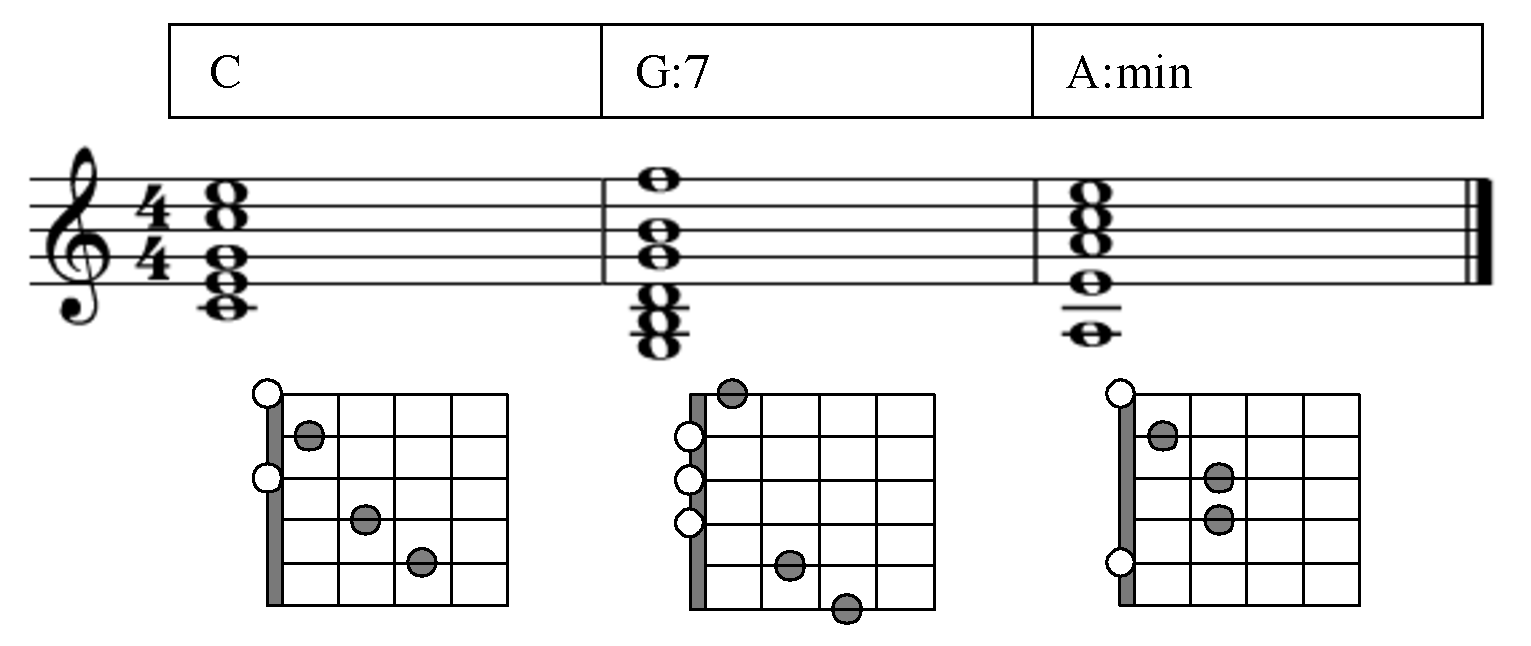
\includegraphics[width=0.8\textwidth]{chord_tablature}}
\caption{A chord sequence (top), traditional staff notation (middle), and guitar tablature (bottom) of the same musical information, in decreasing levels of abstraction.}
\label{fig:chord_notation}
%
\end{figure}

% Rise of the guitarists
To date, the majority of research in automatic chord estimation is based on the two-fold premise that (a) it is fundamentally a classification problem, and (b) the ideal output is a time-aligned sequence of singular chord names.
That said, it is worthwhile to reconsider how the development of such systems is motivated by the goal of helping the ambitious musician learn to play a particular song.
Notably, guitarists comprise one of the largest groups of musicians attempting to do just that.
Over the last century, the guitar, in all of its forms, has drastically risen in popularity and prevalence, both in professional and amateur settings.
Given the low start-up cost, portability, favorable learning curve, and ---courtesy of musicians like Jimi Hendrix or \emph{The Beatles}--- an undisputed ``cool factor'' in Western popular culture, it is unsurprising that guitars dwarf music instrument sales in the United States.
Based on the 2014 annual report of the National Association of Music Merchants (NAMM), a whopping 2.47M guitars were sold in 2013 in the United States, accounting for a retail value of \$1.07 \emph{billion} USD \cite{NAMM2014Global}; as a point of comparison, all wind instruments \emph{combined} ---the next largest instrument category--- totaled just over half that figure, at \$521M USD.

% Tablature notation
The fact that guitarists comprise such a large portion of the musician community is important, as it affects how they might prefer to interact with a chord estimation system.
While most instruments make use of traditional staff notation, fretted instruments, like lute or guitar, have a long history of using \emph{tablature} to notate music.
Illustrated in Figure \ref{fig:chord_notation}, tablature requires minimal musical knowledge to interpret, and thus offers the advantage that is easier to read, particularly for beginners.
Whereas staff notation explicitly encodes pitch information, leaving the performer to translate notes to a given instrument, tablature explicitly encodes performance instructions for a given instrument.
Though it can be difficult to accurately depict rhythmic information with tablature, this is seldom an obstacle for guitarists.
Chord-centric guitar parts typically place less emphasis on rhythm, and changes are usually aligned with lyrics or metrical position.

\begin{figure}[t!]
  \centering
  \centerline{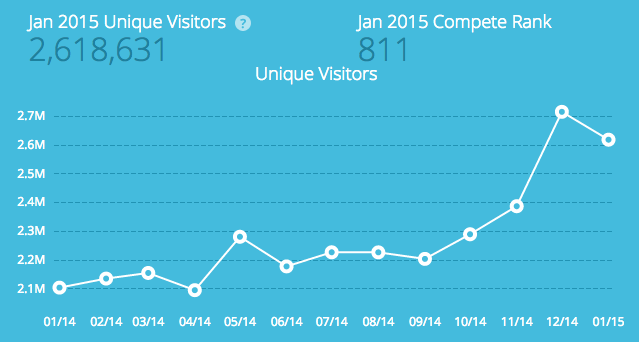
\includegraphics[width=0.8\textwidth]{ug_compete}}
\caption{Visitor statistics for the tab website \emph{Ultimate Guitar}, as of January 2015.}
\label{fig:ug_compete}
%
\end{figure}

% Digitization and the internet
From the earliest days of personal computing, contemporary guitarists have embraced technology en masse for the creation and dissemination of ``tabs.''
Initial bandwidth and memory limitations, however, prevented the curation of high resolution images of sheet music, and symbolic representations, like MIDI, required specialized programs to render the music visually.
With small file sizes and compatibility with common text editors, ASCII ``tabs'' made it comparatively trivial to create, share, and store guitar music.
Thus, combining easy readability and a sufficient level of musical detail with technological constraints of the time period, guitar tablature spiked in popularity towards the end of the $20^{th}$ century.
As evidenced by heavily trafficked, user-curated websites like Ultimate Guitar\footnote{http://www.ultimate-guitar.com/}, modern online guitar communities continue to place a high demand on tablature.
Shown in Figure \ref{fig:ug_compete}, this website alone sees, on average, over 2M unique visitors\footnote{Based on Compete.com analytics data, accessed on 15 March, 2015.} per month in the United States.

% Put it together
Taken together, these observations motivate an obvious conclusion.
Guitarists comprise a significant portion of the global music community, and are actively creating and using tablature as a means of learning music.
An automatic chord estimation system would be extremely valuable to this demographic, but such a system should be sensitive to the common preference for tablature.
Therefore, this chapter is an effort to steer automatic chord estimation toward a specific application, in order to address a potential use case for a very real demographic.


\section{Proposed System}

Building on previous efforts in automatic chord estimation, the best performing configuration presented in Chapter 5, XL-0.125, is extended here for guitar chord estimation.
As such, many design decisions remain consistent with the previous description, such as the constant-Q representation, dataset, or evaluation methodology, and are omitted from the discussion.
There are a few important differences, however, which are addressed below.
First, the architecture is modified slightly to produce fretboard-like outputs.
A strategy is then discussed for incorporating guitar chord shapes into the model.
The modified objective and decision functions are presented last, detailing how the model is optimized and used to estimate discrete chord classes.

Finally, it is worth mentioning that, despite the desire to map notes to a guitar fretboard, this approach is much closer in principle to chord estimation than automatic transcription methods.
Thus, while some previous work embraces this position in the realm of transcribing guitar recordings \cite{Barbancho2012Automatic} or arranging music for guitar \cite{Hori2013Input}, the only previous work in estimating guitar chords as tablature directly from polyphonic recordings is performed by the author, in \cite{Humphrey2014Music}.


\subsection{Designing a Fretboard Model}
\label{subsec:design}

So far, this study has shown deep trainable networks to be a powerful approach to solving complex machine learning problems.
Another particular advantage of deep learning is that it can be remarkably \emph{flexible}, whereby functionally new systems can be developed quickly by making different architectural decisions\footnote{
Provided its ``quality'' can be expressed as a differentiable objective function, that is, and there exists adequate training data.}.
This high-level design strategy is exploited here by modifying the convolutional neural network used in the previous chapter to produce an output representation that behaves like the fretboard of a guitar.

To understand the proposed model, it is helpful to first review the physical system of interest.
The modern guitar consists of six parallel strings, conventionally tuned to E2, A2, D2, G3, B3, and E4, and thus can simultaneously sound between zero and six notes.
A guitar is also fretted, such that the different pitches produced by a string are quantized in ascending order as a function of fret, resulting from shortening the length of the vibrating string in discrete quantities.
Continuous pitch may be achieved by various means, such as bending the strings, but such embellishments are beyond the scope of consideration here.
Thus, it can be said that each string only takes a finite number of states: off (\texttt{X}), open, (\texttt{O}), or a number corresponding to the fret at which the string is held down.
Most real guitars have upwards of 20 frets, but, as a simplification, all chords will be voiced in the first seven frets;
therefore, in this model, each string will take one of nine mutually exclusive states.

Framed as such, the strings of a guitar can be modeled as six correlated, but functionally independent, probability mass functions.
This is achieved by passing the output of an affine projection through a softmax function, as described in Chapter \ref{chp:deep_learning}, yielding a non-negative representation with unity magnitude.
Starting with the first three layers of the ``XL'' model defined previously, six independent softmax layers are used to model each string independently, and concatenated to form a 2-dimensional heatmap of the fretboard:

\begin{align*}
\label{eq:softmax_layer}
\small
Z_i = f_i(X_{l-1} \vert \theta_i) = \sigma (W_i \bullet X_{l-1} + b_i), i \in [0:6), \theta = [W_i, b_is]
\end{align*}

\noindent The activation of the $i^{th}$ string, $Z_i$, is computed by projecting the output of the penultimate layer, $X_{L-1}$, of an $L$-layer network against the weights, $W_i$, and added to a bias term, $b_i$.
This linear transformation is normalized by the softmax function, $\sigma$, and repeated for each of the six strings.
The overall model is diagrammed in Figure \ref{fig:guitarnet}.

\begin{figure}[t!]
  \centering
  \centerline{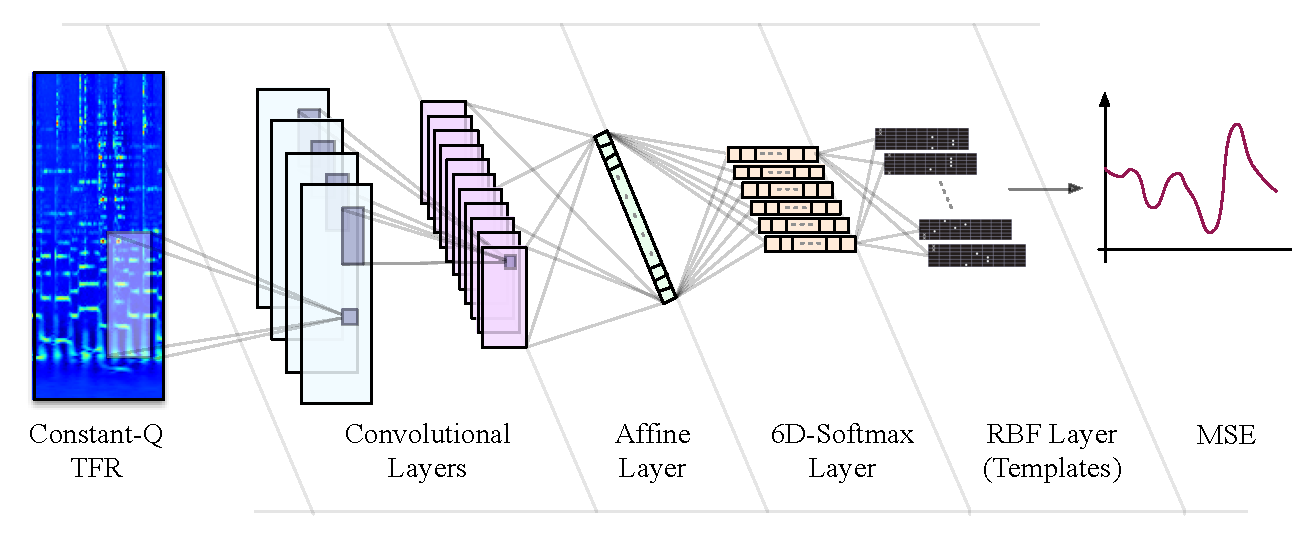
\includegraphics[width=\textwidth]{sys_diagram}}
\caption{Full diagram of the proposed network during training.}
\label{fig:guitarnet}
%
\end{figure}


\subsection{Guitar Chord Templates}
\label{subsec:vocabulary}

Having designed a convolutional network to estimate the active states of a fretboard, it is necessary to devise a mapping from chord transcriptions to fingerings on a guitar.
As the annotations available were curated for generic chord estimation, they  do not offer insight into how a given chord might best be voiced on a guitar.
Therefore, using the same vocabulary of 157 chords as before, a canonical chord shape ``template'' is chosen for each.
This is done in such a way so as to prefer voicings where all quality variations over a given root are maximally similar, i.e. chords of the same root are near-neighbors in fretboard space.
%To illustrate, tablature representations for all templates are given in Figure \ref{fig:templates}.

It is worthwhile at this point to acknowledge the natural multiplicity of chord voicings on the guitar.
In addition to the normal variation that may occur in stacking the notes of a chord, e.g. ``open'' or ``closed'' position, there are other factors that influence the actual pitches that are played.
First, the same note can often be played in multiple positions on the fretboard.
For example, E3 can be played on the 12th fret of the first string, the 7th of the second, or the 2nd of the third.
Additionally, some standard chord voicings cannot be formed on the guitar, comfortably or otherwise.
For this reason it is quite common to play the 3rd scale degree of a chord above the octave, as the 10th, though there are a few exceptions resulting from open fingerings.
Context may also influence how a chord is played, such as the instance in which it is easier to move from one chord shape to the next.
Rather than attempt to address all of these issues now, the canonical template approach is chosen as a practical means to simplify overall system design.
The choice of one template over another likely has nontrivial implications for the behavior of the model, but this is identified as a opportunity for future inquiry.


\subsection{Decision Functions}
\label{subsec:loss}

While estimating frets is sufficient for human interpretation, it is necessary to design two related decision functions in order to allow the machine to operate automatically.
First, the templates defined above must be incorporated into an objective function, such that the machine can learn to optimize this measure over the training data.
Finding inspiration in \cite{LeCun1998Gradient}, a Radial Basis Function (RBF) layer is added to the network, given as follows:

\begin{equation}
\small
\mathcal{E}(Z \vert W_T) = \sum(Z_{out} - W_{T}[k])^2
\end{equation}

\noindent where $Z$ is the output of the fretboard model, $W_T$ is a tensor of chord shape templates with shape $(K, 6, 9)$, such that $K$ is the number of chord templates, and $k$ the index of the reference class.
Note that these templates will impose the proper organization on the output of the model, and thus remain fixed during the learning process.
Since these weights are constant, minimizing this function does not require a contrastive penalty or margin term to prevent it from collapsing, i.e. making all the squared distances zero.

Additionally, for the purposes of Viterbi post-filtering and fairly comparing with previous results, the energy surface must be inverted into a likelihood function.
This is achieved by negating the energy function, $E$, and normalizing as a Gibbs distribution:

\begin{equation}
\small
\mathcal{L}(Y_k \vert X, \Theta) = \frac{exp(-\beta~E(Y_k \vert X, \Theta))}{\sum_i^K~exp(-\beta~E(Y_k \vert X, \Theta))}
\end{equation}

For the experiments detailed below, $\beta=1$.
It is conceivable that the choice of hyperparameter may impact system behavior when coupled with the Viterbi algorithm, but this value was empirically observed to give good results and not explored further.


\section{Experimental Method}

The focus of this chapter now shifts toward the experimental method adopted to investigate the behavior of this basic approach.
Herein, the training strategy, corresponding variables, and subsequent quantitative results are addressed in turn.

\subsection{Training Strategy}
\label{subsec:strategy}

Though it is able to incorporate musical knowledge into the architectural design, the model proposed here is unable achieve root-invariant weight sharing as in the previous chapter.
This is due to root-dependent chord shapes resulting from the nonuniform arrangement of chords on the neck of the guitar.
It is important to consider the effect this has on system performance, as well as other means of achieving ``root invariance'', and thus three different training strategies are employed here.

As a baseline condition, the model is trained with the natural distribution of the data (``as-is'').
Note that it is reasonable to expect these models to be deficient, as there may be chord class mismatch between training and test conditions, i.e. chord classes in the test partition do not occur in the training set.
To address the imbalanced learning problem, the second training condition scales the loss of each training observation by a class-dependent weight (``scaled'').
These weights are determined by computing the root-invariant prior over the training partition, taking its inverse, and standardizing the coefficients to unit mean and standard deviation.
The third and final training condition couples loss scaling with data augmentation, such that during training each datapoint is randomly shifted in frequency on the interval $[-12, 12]$ (``augmented'').
This allows the variance of each chord quality to be evenly distributed across classes, and helping prevent any missing class coverage in the training set.

Identical partitions of the dataset used in the previous chapter are employed here; the dataset is split 68:12:20, into training, validation, and test, respectively, and the partitions are rotated so that all data is used as a holdout set once.
All models are trained with mini-batch stochastic gradient descent at a batch size of 100, learning rate of 0.02, and dropout ratio of 0.125.
Training proceeded for several hundred iterations, ultimately bounded by a ceiling of 24 hours, and parameters checkpointed every 10k iterations.
Model selection was performed as a brute force search over both the parameter checkpoints and self-transition penalty for Viterbi, from -20 to -40 in steps of 5.
The best model was chosen by the maximum of the harmonic mean of the chord evaluation metrics outlined previously.


\subsection{Quantitative Evaluation}
\label{subsec:evaluation}

In the absence of a thorough user study, the proposed approach is evaluated against the chord estimation task posed in Chapter 5.4.
Applying the methodology outlined above, the three training conditions were run to completion and used to predict into the space of 157 chord classes.
Given the intersection with the previous chapter, these three systems are compared to the system presented in \cite{Cho2014Improved}, referred to as ``Cho'', and the model related to those explored here, ``XL-0.125'', referred to now as the ``root-invariant'' condition.

\begin{table}[t]
\begin{center}
\scriptsize
\caption{Weighted recall scores over the test set for two previous models, and the three conditions considered here.}
\label{tab:test_micro}
\begin{tabular}{c|rrrrrrr}

\hline
 & triads &   root &   MIREX &   tetrads &   sevenths &   thirds &   majmin \\
\hline
Cho & 0.7970 & 0.8475 & 0.8147 & 0.6592 & 0.6704 & 0.8197 & 0.8057 \\
\hline
Root-invariant (Chapter 5)  & 0.7995 & 0.8493 & 0.8145 & 0.6673 & 0.6788 & 0.8227 & 0.8077 \\
\hline
As-Is     & 0.8234 & 0.8705 & 0.8352 & 0.6855 & 0.7084 & 0.8376 & 0.8394 \\
Scaled    & 0.8156 & 0.8644 & 0.8283 & 0.6791 & 0.6994 & 0.8308 & 0.8295 \\
Augmented & \textbf{0.8294} & \textbf{0.8715} & \textbf{0.8420} & \textbf{0.6989} & \textbf{0.7167} & \textbf{0.8440} & \textbf{0.8412} \\
\hline
\end{tabular}
\end{center}
\end{table}

Overall performance is measured as weighted recall across metrics, as per the previous chapter, and given in Table \ref{tab:test_micro}.
These results indicate that, over all the data, the three fretboard models perform far better than either of the two previous ones.
Additionally, the combination of weight scaling and pitch shifting leads to the best overall performance.
As the second, weight-scaled condition fares slightly worse than training the models with the data as-is, there is reason to conclude that applying pitch shifting only during training will likely result in higher overall scores.
This inquiry is left as an opportunity for future work.


\begin{table}[t]
\begin{center}
\scriptsize
\caption{Quality-wise recall across conditions.}
\label{tab:test_qualitywise}
\begin{tabular}{c|c|ccc|c}

 quality   &  Root-invariant &  As-is & Scaled & Augmented & Support (min) \\
\hline
 maj       &  0.7390 &  0.8572 &  0.8413 &  0.8417 &  397.4887 \\
 min       &  0.6105 &  0.6516 &  0.6312 &  0.6645 &  105.7641 \\
 7         &  0.5183 &  0.2928 &  0.3001 &  0.3367 &   68.1321 \\
 min7      &  0.5263 &  0.4556 &  0.4670 &  0.5077 &   63.9526 \\
 N         &  0.7679 &  0.6670 &  0.6712 &  0.6942 &   41.6994 \\
 maj7      &  0.6780 &  0.4143 &  0.4614 &  0.5525 &   23.3095 \\
 \hline
 maj6      &  0.2908 &  0.0259 &  0.0682 &  0.1061 &    7.6729 \\
 sus4      &  0.3369 &  0.0252 &  0.0952 &  0.1747 &    8.3140 \\
 sus2      &  0.3216 &  0.0098 &  0.0146 &  0.2216 &    2.4250 \\
 aug       &  0.5078 &  0.0093 &  0.1431 &  0.3365 &    1.2705 \\
 dim       &  0.4105 &  0.2898 &  0.4030 &  0.3803 &    1.8756 \\
 min6      &  0.3870 &  0.0367 &  0.1611 &  0.3011 &    1.5716 \\
 hdim7     &  0.5688 &  0.0000 &  0.0610 &  0.3913 &    1.1506 \\
 dim7      &  0.1790 &  0.0040 &  0.0453 &  0.0391 &    0.5650 \\
 \hline
 average   &  0.4887 &  0.2671 &  0.3117 &  0.3963 &  \\
\hline
\end{tabular}
\end{center}
\end{table}

However, quality-wise recall, given in Table \ref{tab:test_qualitywise}, offers a more nuanced depiction of the effect of these strategies.
Going from the ``as-is'' to ``scaled'' conditions, the slight reduction in micro-recall is traded for an increase in averaged quality-wise recall.
This result is intuitively satisfying, as the introduction of class-dependent weights into the training process should help raise the preference for the long tail chords.
Though this can help attenuate the model's strong preference for majority chord classes, it does nothing to help address the overall deficiency of minority classes.
Therefore, when loss scaling is combined with data augmentation, the increase in performance is profound; nearly all statistics, at both the micro and quality-wise macro level, improve, some significantly.

Additionally, it can be seen that the higher overall scores in the guitar model are a result of over-predicting majority, and in particular ``major'', chords.
Compared to the root-invariant model of the previous chapter, the guitar models are over 10\% better at predicting major chords alone.
Somewhat surprisingly, the root-invariant model is nearly 20\% better at dominant seven chords than any new model trained here.
This can be understood as an artifact of the intersection in fretboard space between major and dominant seven chords, coupled with the significant bias toward major chords.
Finally, as to be expected, the imbalanced distribution of chord qualities prevents the lower quality-wise scores from being reflected in the overall, micro-recall statistics.
This behavior alludes to the previous discussion regarding the apparent trade-off between global performance and quality-wise accuracy.


\begin{figure}[t!]
  \centering
  \centerline{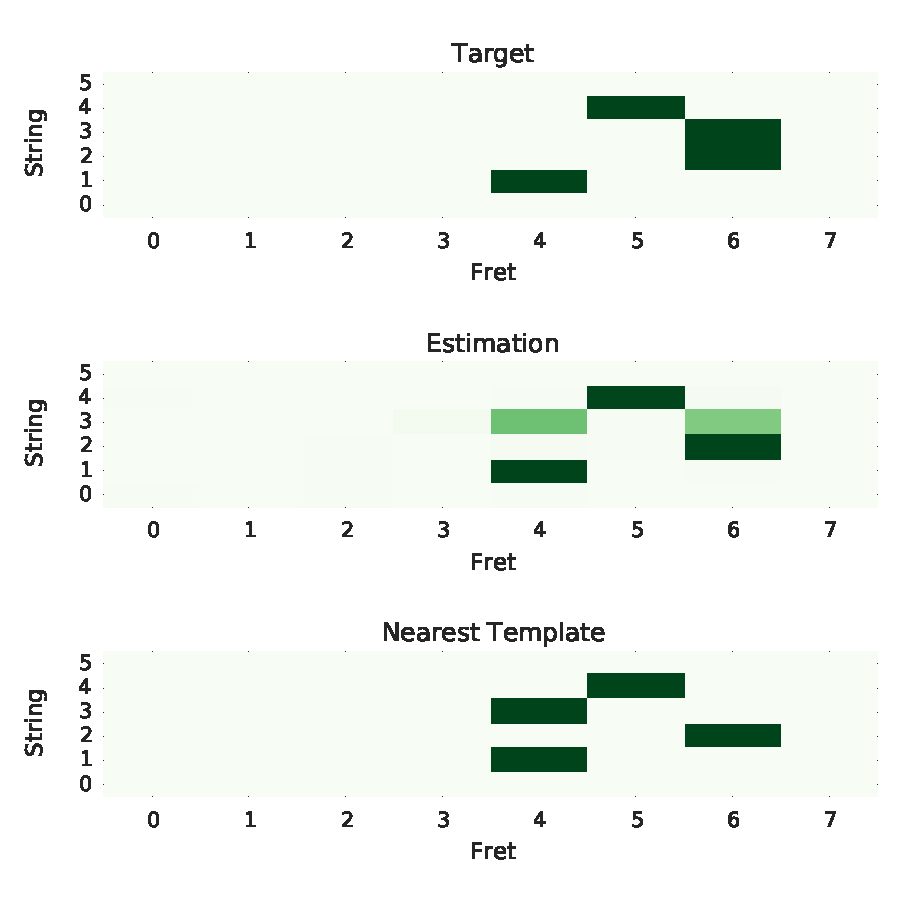
\includegraphics[width=0.8\textwidth]{quantized}}
\caption{Understanding misclassification as quantization error, given a target (top), estimation (middle), and nearest template (bottom).}
\label{fig:quantized}
%
\end{figure}


Another important behavior to consider here is the idea that the direct estimation of a fretboard representation affords some benefit over simply projecting the predicted labels of a standard chord classifier \emph{back} onto guitar chord templates.
Typical chord estimation systems, and especially those that rely heavily on Viterbi, like \cite{Cho2014Improved}, produce a sequence of discrete chord labels, and are thus effectively ``classifiers''.
Comparatively, fretboard estimation can be seen as regression, given the continuous output surface, but can be used for classification by identifying the closest known chord template, referred to as \emph{vector quantization}.
Thus, illustrated in Figure \ref{fig:quantized}, misclassification can be understood as a type of quantization \emph{error};
here a prediction close to, but on the wrong side of, the decision boundary is assigned to a different chord shape.
However, since the representation is human readable, it is trivial to correct the error from a \texttt{C\#:min7} to \texttt{C\#:min}.


\begin{figure}[t!]
  \centering
  \centerline{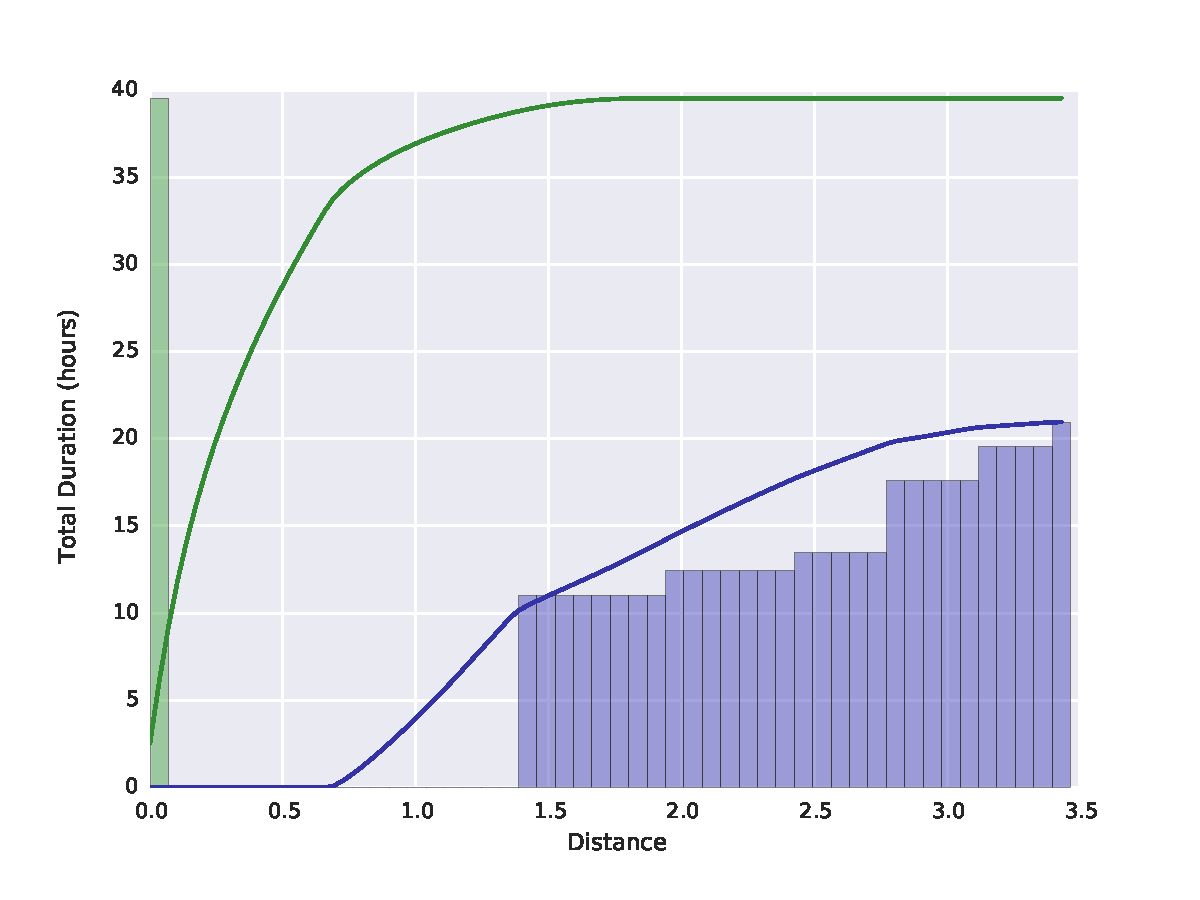
\includegraphics[width=0.8\textwidth]{quant_error}}
\caption{Cumulative distribution functions of distance are shown for correct (green) and incorrect (blue) classification, in the discrete (classification) and continuous (regression) conditions.}
\label{fig:quant_error}
%
\end{figure}

In the space of fretboard estimation, this can be quantified by comparing the distances between predictions and the ideal template both before and after classification, partitioned on whether or not the datapoint is correctly assigned.
First, the distances between the continuous-valued fretboard and the corresponding target template are computed and tallied as two histograms, partitioned on binary accuracy and normalized by the total number of observations.
Next, the estimated fretboard representations are assigned to the \emph{nearest} template, and distance is computed to the target;
these distances are also histogrammed, split on correctness, but take only a few discrete values due to the vector quantization introduced by classification.
These four density functions are then integrated into continuous distribution functions (CDF).
Shown in Figure \ref{fig:quant_error}, these CDFs can be understood as representing the ratio of total observations as a function of an estimation's distance from the ideal representation.
Here, it can be seen that misclassification effectively widens the gap between correct and incorrect answers.
Alternatively, in the regression scenario, nearly 20\% of these errors are ``closer'' to their correct class's template, accounting for well over 80\% of the data.
Importantly, this additional information, contained in an incorrect prediction, is precisely what makes it easier for potential users to correct mistakes;
they are offered insight into \emph{how} the system may have failed.


\section{Discussion}

This chapter has proposed a method of extending a previous automatic chord estimation by introducing the physical constraints of a guitar.
Not only does this yield a higher performing system, based on overall metrics, but the outputs are directly human readable making the system attractive from a user experience standpoint.
While the system seems to struggle more than previous efforts across all chord qualities, this is arguably an instance in which performing better over \emph{all} the data is preferable.
The sample sizes of rare chords in the dataset are at times too small to draw meaningful conclusions about performance at the class level.
Further complicating matters, there is also some unknown degree of subjectivity in the reference annotations, used for both training and evaluation.
Pragmatically speaking though, consistently tracking root motion, e.g. being in the right place on the neck, is probably sufficient for most guitarists to deem such a system useful.
The vast majority of music can be simplified as ``power chords'', consisting of the root and the fifth, and often more detailed chords can be realized by modifying this basic shape.
Therefore, while many methodological challenges inherent to chord estimation persist in this study, predicting chord shapes as tablature softens the degree to which they impact usability.

Setting aside the limitations of quantitative evaluation in chord estimation, the proposed system warrants a subjective, user experience study in the future.
Many of the gains identified here can only be qualitatively assessed by how such a system achieves its goals, such as the degree to which performance \emph{does} in fact degrade gracefully.
Countless instances can be identified where system ``errors'' can be reasonably interpreted as the chord name provided, but only a study with real users will indicate how useful this is.

Perhaps most importantly though, the next logical research step is to develop an interactive user interface and deploy such a system at scale.
In addition to distributed instruction, deploying an ``autotabbing'' system provides a means to collect and clean reference annotations.
Approaching this task from the perspective of human-readable representations holds considerable promise in the space of data curation, as editing a chord transcription is generally a far simpler task than creating one from scratch.
This reality is only amplified for annotators who lack formal ear training.
Importantly though, this reduces the prerequisite skill level, the amount of time needed to complete the task, or both, required in the data authoring task.
Therefore, this system creates the potential to include a larger number of musicians across a wide array of skills in the data collection process.
More annotators not only opens the door for more annotations, but multiple perspectives of the \emph{same} music content.
This will be critical to the role subjectivity plays in chord estimation research, now and in the near future.


